
In this article, we cover a diverse range of 
{\em system relaxations} techniques for 
distributed stochastic gradient descent systems.
From a mathematical optimization perspective, all
system relaxations we introduce {\em does not
make the convergence (loss vs. \# iterations / epochs) faster}.
\footnote{The reason
that we emphasize the ``mathematical optimization''
perspective is because that some researchers
find certain system relaxations can actually lead
to better generalization performance~\cite{XXX,XXX}.
We do not consider generalization in this article.}
%
Then {\em why do we even want to introduce these 
relaxations into our system in the first place?}

One common theme of the techniques we cover in
this article is that their goal is not
to improve the convergence rate in terms
of \# iterations / epochs, but instead, their
goal is to make each iteration finishes faster
in terms of wall clock time.
As a result, to reason about each system relaxation
techniques in this article, we need to first
agree on a {\em performance model} of the
underlying distributed system. In this Section,
we introduce a very simple performance model --- 
it ignores many (if not most) important system
characteristics, but is just informative enough
for readers to understand why each system relaxations
in this article actually makes a system faster.

\subsection{Assumptions}

\begin{figure}[t!]
\centering
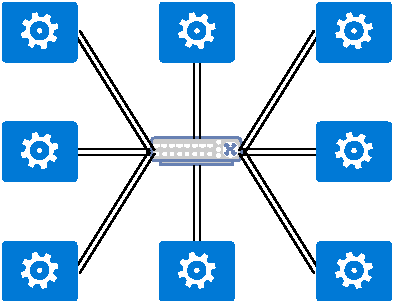
\includegraphics[width=0.3\textwidth]{figures/Chpt1.3/CommunicationModel.pdf}
\caption{An illustration of the distributed communication
model we use in this article. We assume that all devices
(worker, machine) are connected via a ``logical switch'',
whose property is defined in Section~\ref{sec:commmodel}}.
\label{fig:commmodel}
\end{figure}

Figure~\ref{fig:commmodel} illustrates our communication model. Each worker (blue rectangle)
corresponds to {\em one} computation device,
and all workers are connected via a ``logical switch''
that has the following property:
\begin{enumerate}
\item The switch has infinitely large bandwidth.
\item For each message that ``passes through''
the switch (send by worker $w_i$ and received
by worker $w_j$), the switch adds a constant
delay $t_{latency}$ independently of the number
of concurrent messages that this switch is 
serving. This delay is the difference
between the sender sending out the first bit
and the receiver receiving the first bit.
\end{enumerate}

For each worker, we also assume the following properties:
\begin{enumerate}
\item Each worker can only send one message 
at the same time.
\item Each worker can only receive messages 
at the same time.
\item Each worker can concurrently receive one 
message and send one message at the same time.
\item Each worker has a fixed bandwidth, i.e.,
to send / receive one unit (e.g., MB) amount of data,
it requires $t_{transfer\_1MB}$ seconds.
\end{enumerate}

\begin{figure}[t!]
\centering
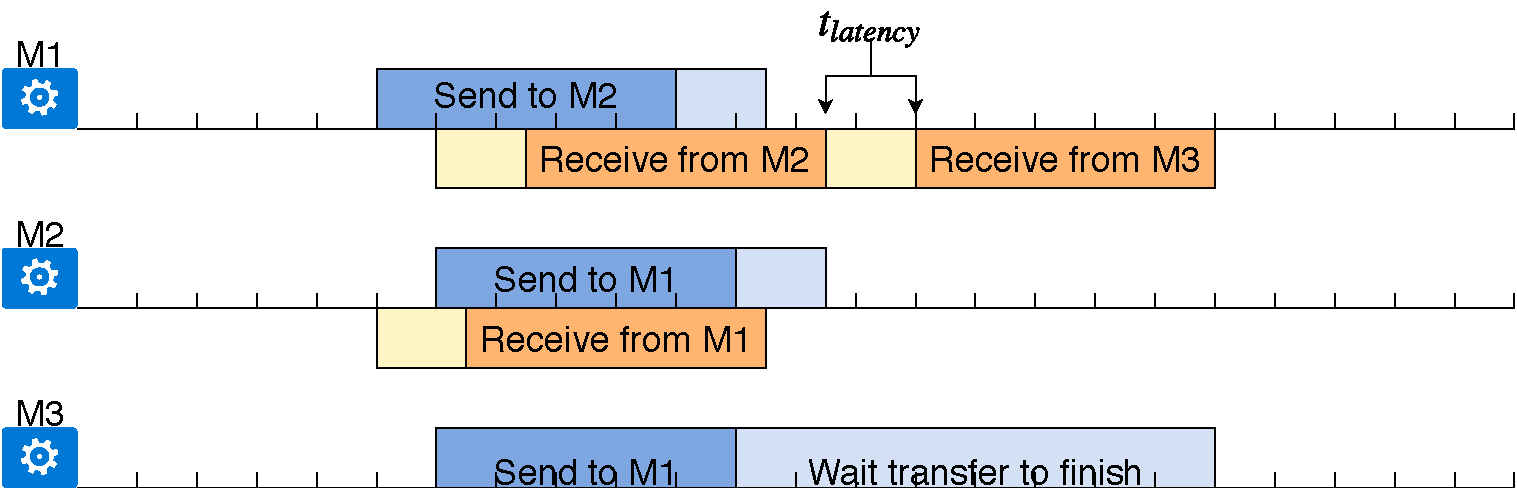
\includegraphics[width=1.0\textwidth]{figures/Chpt1.3/Communication_Illustration.pdf}
\caption{Illustration of the communication pattern of Example~\ref{exp:communication_illustration}.}
\label{fig:communication_illustration}
\end{figure}

\begin{figure}[t!]
\centering
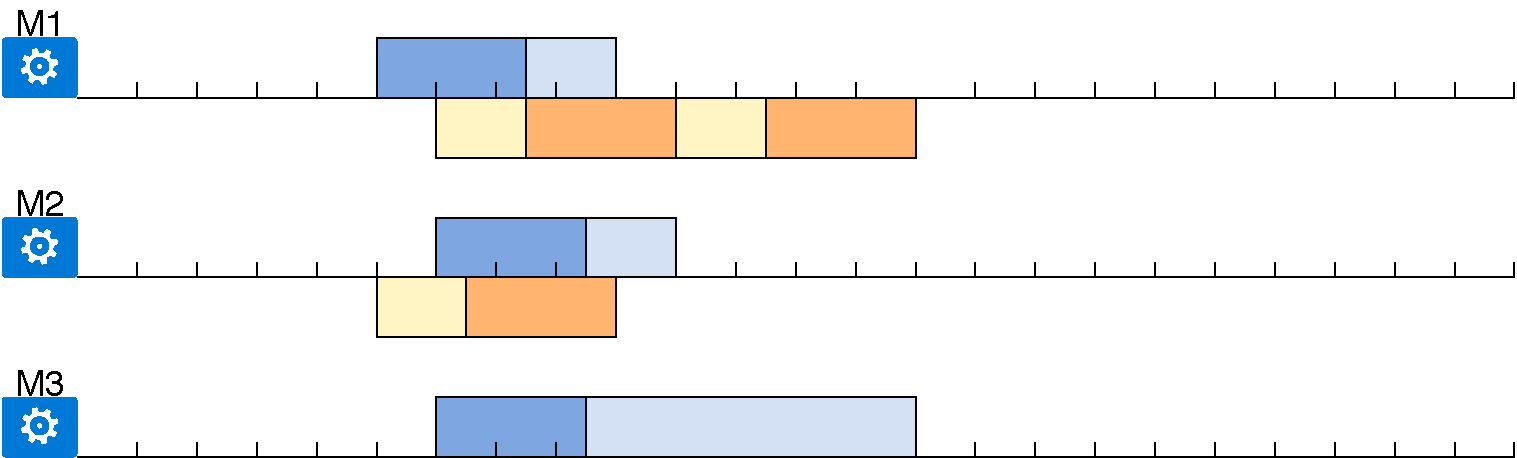
\includegraphics[width=1.0\textwidth]{figures/Chpt1.3/Communication_Illustration_lowPrecision.pdf}
\caption{Illustration of the communication pattern of Example~\ref{exp:communication_illustration}, with 2x data compression.}
\label{fig:communication_illustration_lowprecision}
\end{figure}

\begin{example} \label{exp:communication_illustration}
Under the above communication model,
Consider the following three events:
\begin{verbatim}
            time      event
            0:05      M1 send 1MB to M2
            0:06      M2 send 1MB to M1
            0:06      M3 send 1MB to M2
\end{verbatim}
We assume that the latency added by the switch $t_{latency}$
is 1.5 unit of time and it took 5 units of time to
transfer 1MB of data. 
Figure~\ref{fig:communication_illustration} illustrates 
the timeline on three machines under our communication 
model. The yellow block corresponds to the {\em latency}
added by the ``logical switch''. We also see that 
the machine \texttt{M1} can concurrently send (blue
block) and
receive data (orange block) at the same time; however,
when the machine \texttt{M3} tries to send data to
\texttt{M1}, because the machine \texttt{M2} is
sending data to \texttt{M1} already, \texttt{M3}
needs to wait (the shallow blue block of \texttt{M3}).
\end{example}

\begin{example} \label{exp:communication_illustration}
Figure~\ref{fig:communication_illustration_lowprecision}
illustrates a hypothetical scenario in which 
all data sent in Example~\ref{exp:communication_illustration}
are ``magically'' compressed by 2$\times$ at the sender.
As we will see in later chapters, this is similar to what 
would happen if one compresses the gradient by 2$\times$
during training.

We make multiple observations from Figure~\ref{fig:communication_illustration_lowprecision}.
\begin{enumerate}
\item First, compressing data does make the ``system'' faster.
Without compression, all three events finish in 14 units
of time (Figure~\ref{fig:communication_illustration})
whereas it finishes in 9 units of time after compress.
This is because the time used to {\em transfer}
the data is decreased by half, in our communication model.
\item Second, even if the data are compressed by 2$\times$,
the speedup of the system is smaller than that, in fact, it
is only $14/9 = 1.55\times$. This is because that, even 
though the transfer time is cut by half, the communication
latency does not decrease as a result of data compression.
\end{enumerate}
\end{example}

We now use the above communication model to describe
three popular ways of implementing distributed stochastic 
gradient descent. These implementations will often serve
as the baseline on which we apply different system relaxations
to remove certain system bottlenecks that raise in 
different configurations of $(t_{latency}, t_{transfer})$
together with the relative computational cost on each machine.

\begin{figure}[t!]
\centering
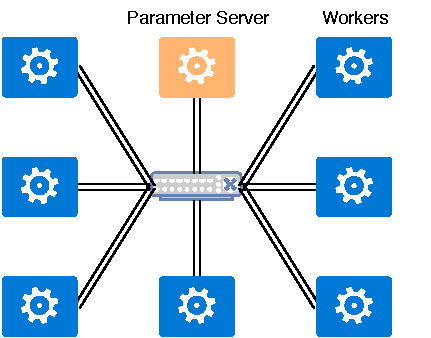
\includegraphics[width=0.3\textwidth]{figures/Chpt1.3/Communication_PS1.pdf}
\caption{Illustration of the parameter server architecture 
with a single dedicated parameter server.}
\label{fig:communication_illustration_ps1}
\end{figure}


\begin{figure}[t!]
\centering
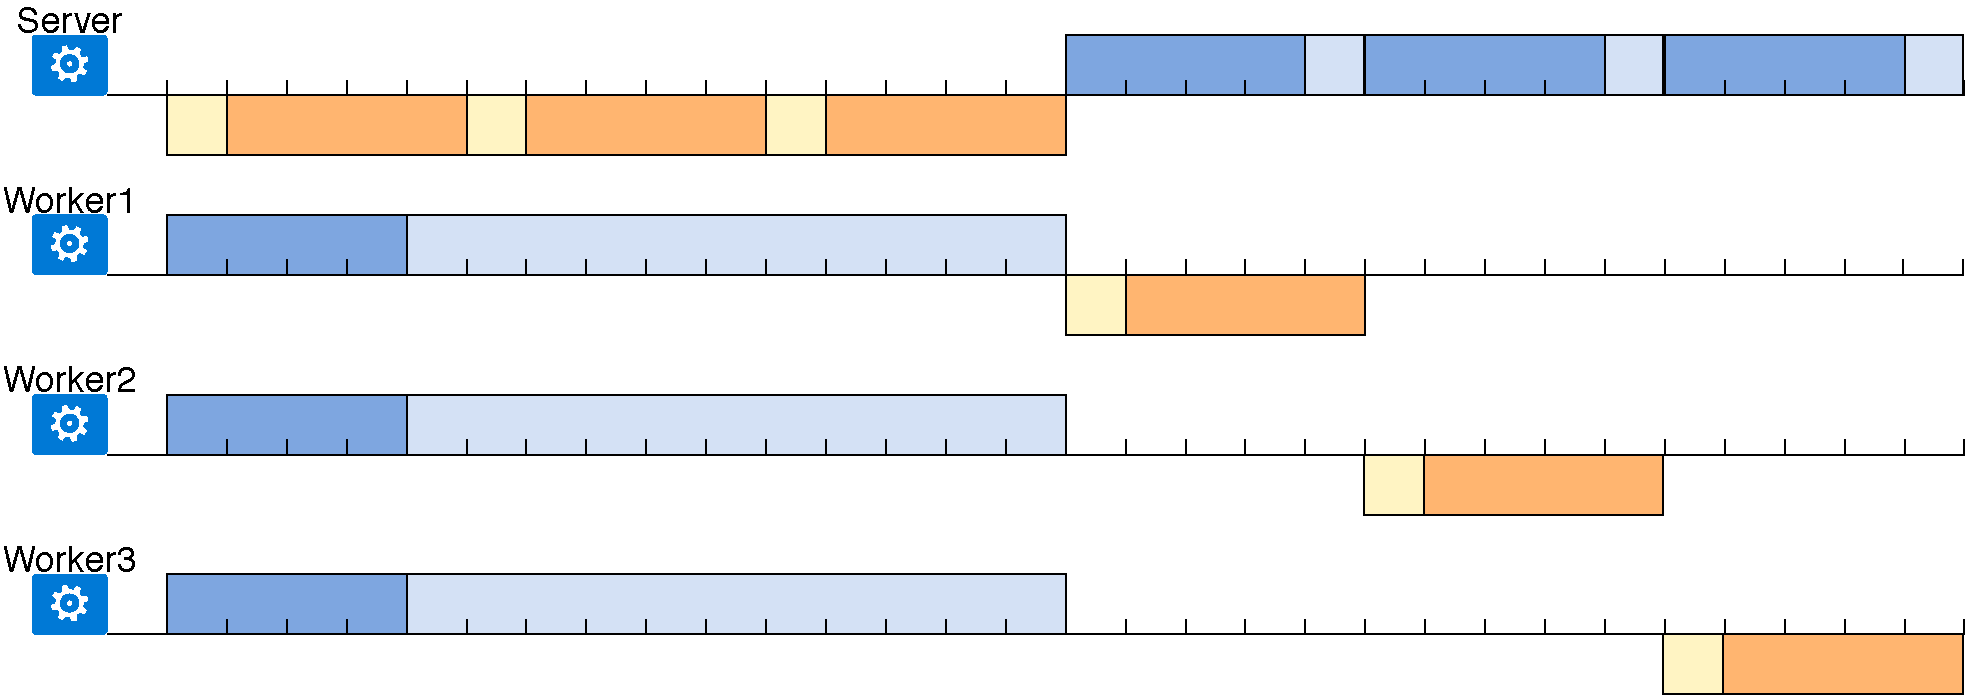
\includegraphics[width=1.0\textwidth]{figures/Chpt1.3/Communication_PS.pdf}
\caption{Illustration of the communication
pattern of the parameter server architecture 
with a single dedicated parameter server.}
\label{fig:communication_illustration_timeline_ps1}
\end{figure}


\begin{figure}[t!]
\centering
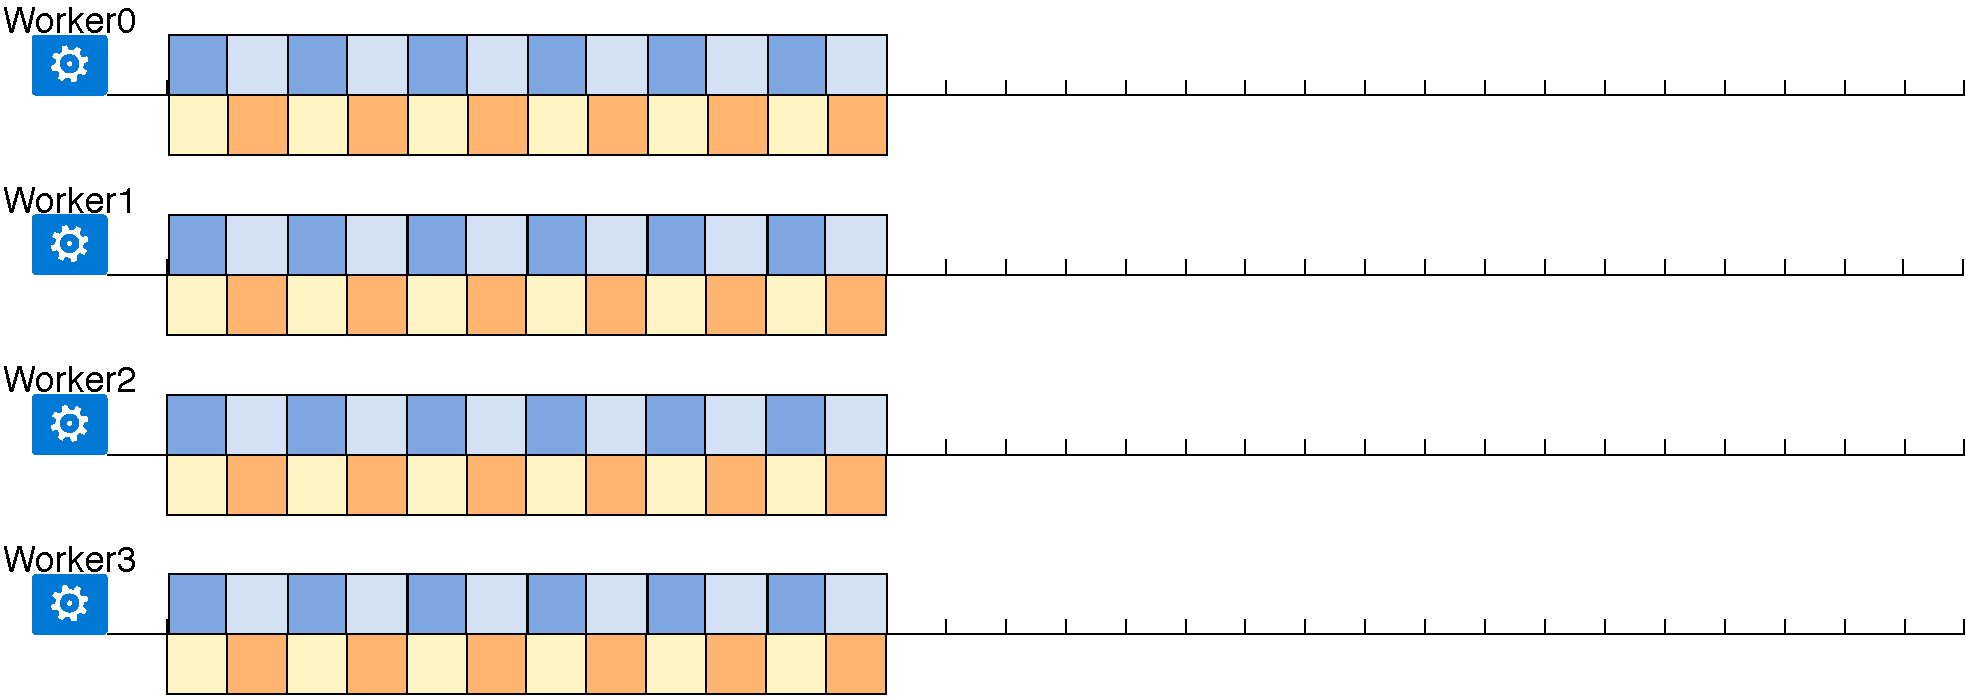
\includegraphics[width=1.0\textwidth]{figures/Chpt1.3/Communication_pattern_AllReduce.pdf}
\caption{Illustration of the communication
pattern of the AllReduce architecture with ring topology.}
\label{fig:communication_illustration_timeline_allreduce}
\end{figure}


\begin{figure}[t!]
\centering
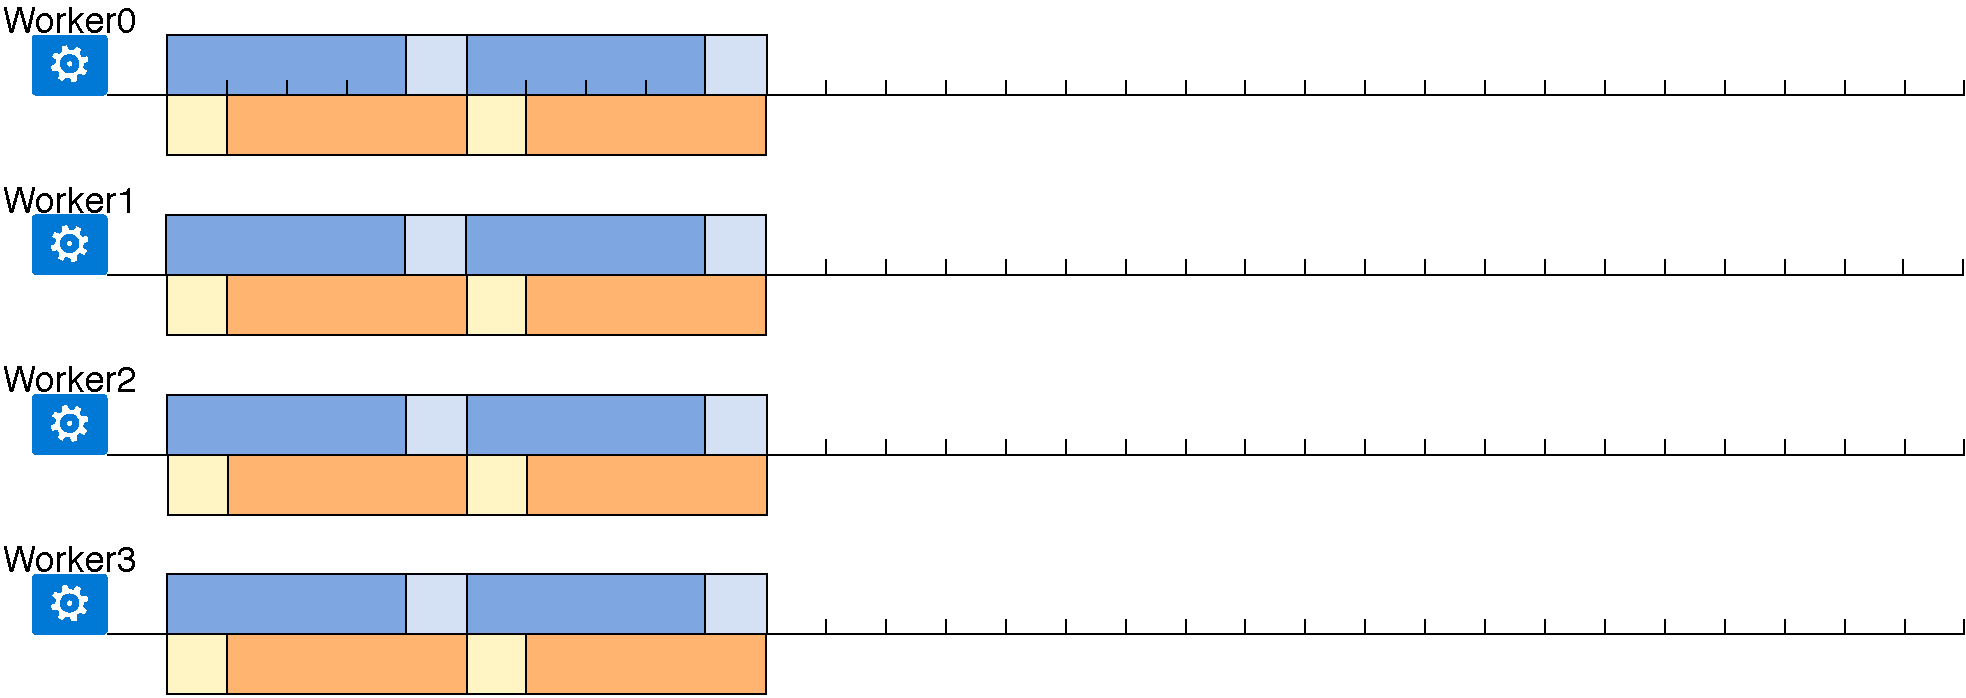
\includegraphics[width=1.0\textwidth]{figures/Chpt1.3/Communication_pattern_decentralized.pdf}
\caption{Illustration of the communication
pattern of the decentralized  architecture with ring topology.}
\label{fig:communication_illustration_timeline_decent}
\end{figure}
\subsection{Parameter Server}

\subsection{AllReduce}

\paragraph{Why Do We Partition the Model?}


\subsection{Multi-machine Parameter Server}








